\documentclass{article}
\usepackage{graphicx}
\usepackage{indentfirst}

\title{Sciences des données - TP2}
\author{Alexandre Theisse \and Louis-Vincent Capelli \and Tom Sartori}

\begin{document}

\maketitle
\newpage

\section*{Question 1}

\subsection*{anger vs happiness}

La représentation conjointe des distributions et la représentation de la 
distribution conjointe des variables 
\textit{anger\_intensity} et \textit{happiness\_intensity}
sont les suivantes :

\begin{center}
    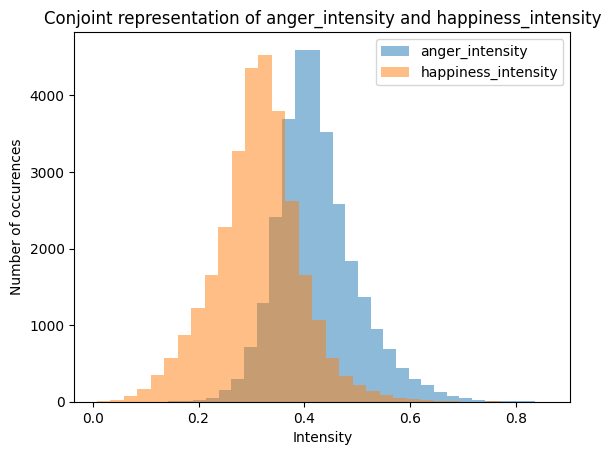
\includegraphics[scale=0.39]{./img/conjoint_representation_anger_intensity_happiness_intensity.png}
    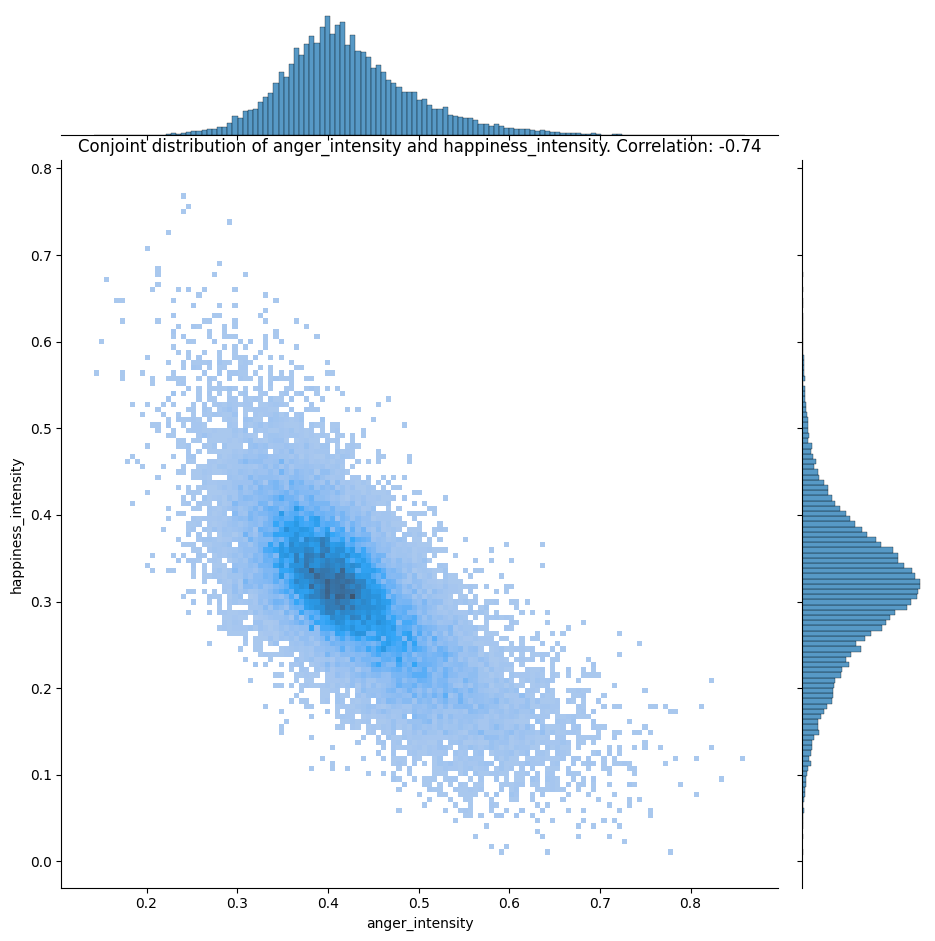
\includegraphics[scale=0.23]{./img/conjoint_distribution_anger_intensity_happiness_intensity.png}
\end{center}

Les distributions sont peu superposées, et la distribution conjointe présente une
anti-corrélation importante (-0.74). On peut donc en conclure que les deux variables jouent
un rôle antagoniste dans la détermination du sentiment de l'internaute et que
généralement seule l'une d'entre elles aura une valeur élevée (par rapport aux valeurs prises
par cette variable en particulier) donnant un sentiment
négatif si \textit{anger\_intensity} est élevée (aux alentours de 0.6) 
et un sentiment positif si
\textit{happiness\_intensity} est élevée (aux alentours de 0.4). Si les deux ont une
valeur similaire, l'internaute pourra être associé à un sentiment neutre.

\subsection*{anger vs sadness}

La représentation conjointe des distributions et la représentation de la
distribution conjointe des variables
\textit{anger\_intensity} et \textit{sadness\_intensity}
sont les suivantes :

\begin{center}
    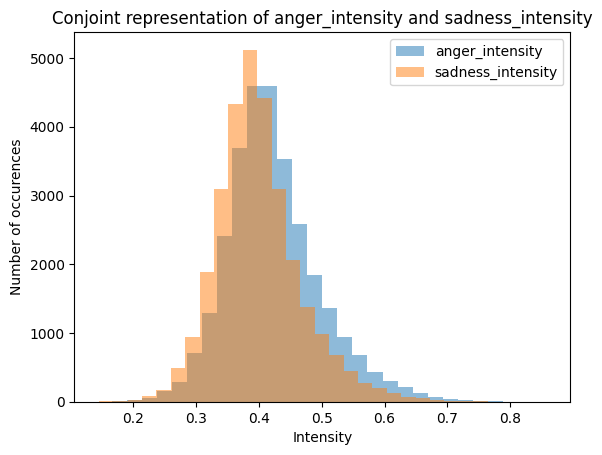
\includegraphics[scale=0.39]{./img/conjoint_representation_anger_intensity_sadness_intensity.png}
    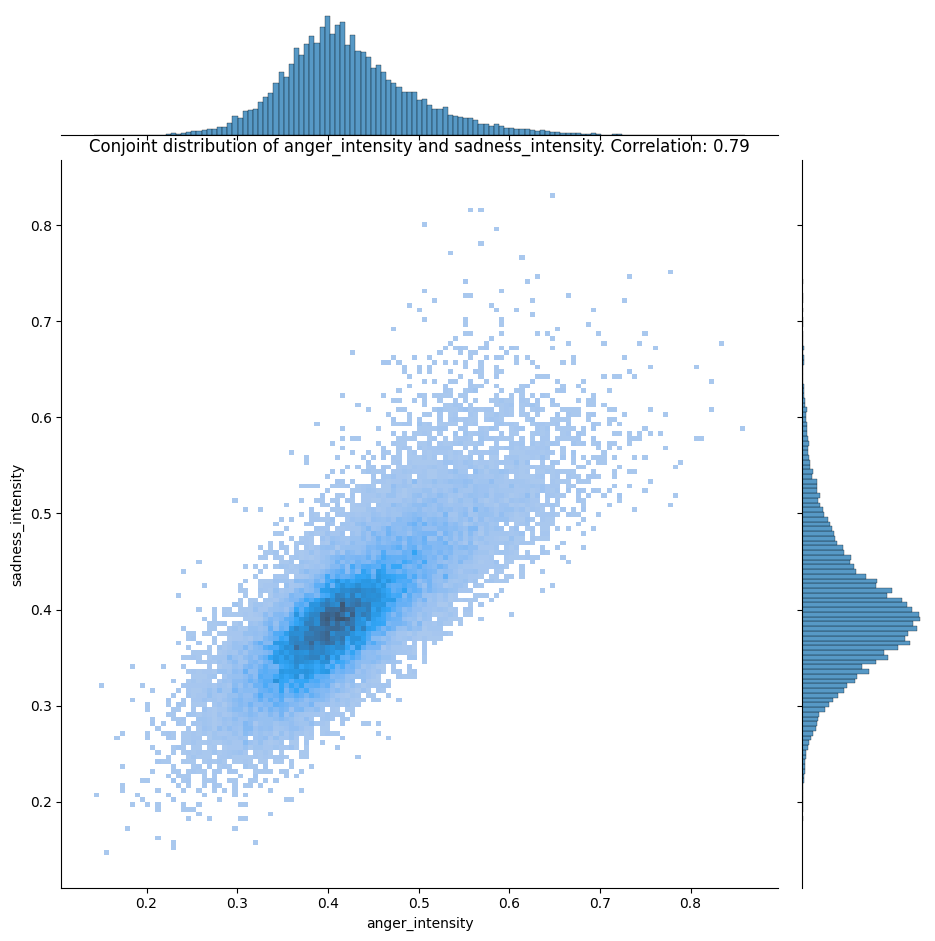
\includegraphics[scale=0.23]{./img/conjoint_distribution_anger_intensity_sadness_intensity.png}
\end{center}

Les distributions sont presque entièrement superposées, et la distribution conjointe
présente une corrélation importante (0.79). On peut donc en conclure que les deux variables
jouent un rôle similaire dans la détermination du sentiment de l'internaute et que
généralement les deux auront une valeur élevée ou faible en même temps. Dans ce cas
précis, on imagine que l'internaute sera associé à un sentiment négatif si les deux
variables ont une valeur élevée et à un sentiment positif si les deux variables ont
une valeur faible.

\subsection*{fear vs anger}

La représentation conjointe des distributions et la représentation de la
distribution conjointe des variables
\textit{fear\_intensity} et \textit{anger\_intensity}
sont les suivantes :

\begin{center}
    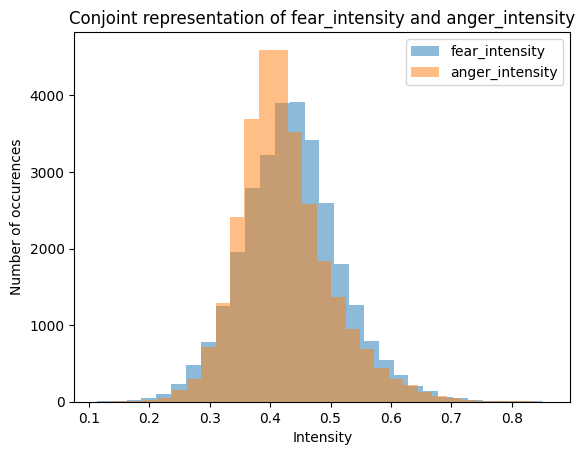
\includegraphics[scale=0.39]{./img/conjoint_representation_fear_intensity_anger_intensity.png}
    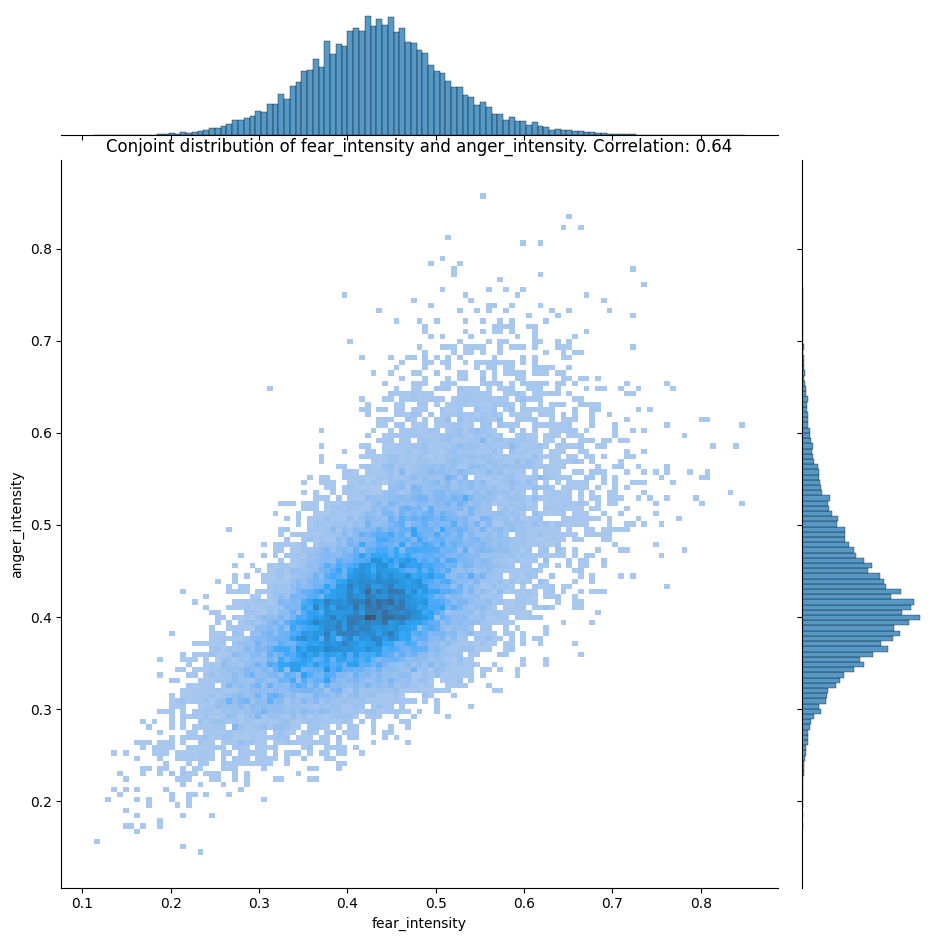
\includegraphics[scale=0.23]{./img/conjoint_distribution_fear_intensity_anger_intensity.png}
\end{center}

Les distributions sont à nouveau très superposées, et la distribution conjointe
présente une corrélation importante (0.64). On peut donc en conclure que les deux variables
jouent un rôle identique dans la détermination du sentiment de l'internaute et que
généralement les deux auront une valeur élevée ou faible en même temps. Dans le cas de
la peur et de la colère, on imagine que l'internaute sera associé à un sentiment négatif.

\subsection*{fear vs happiness}

La représentation conjointe des distributions et la représentation de la
distribution conjointe des variables
\textit{fear\_intensity} et \textit{happiness\_intensity}
sont les suivantes :

\begin{center}
    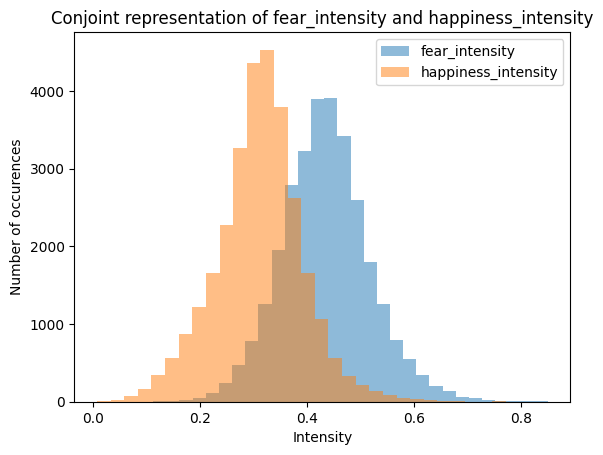
\includegraphics[scale=0.39]{./img/conjoint_representation_fear_intensity_happiness_intensity.png}
    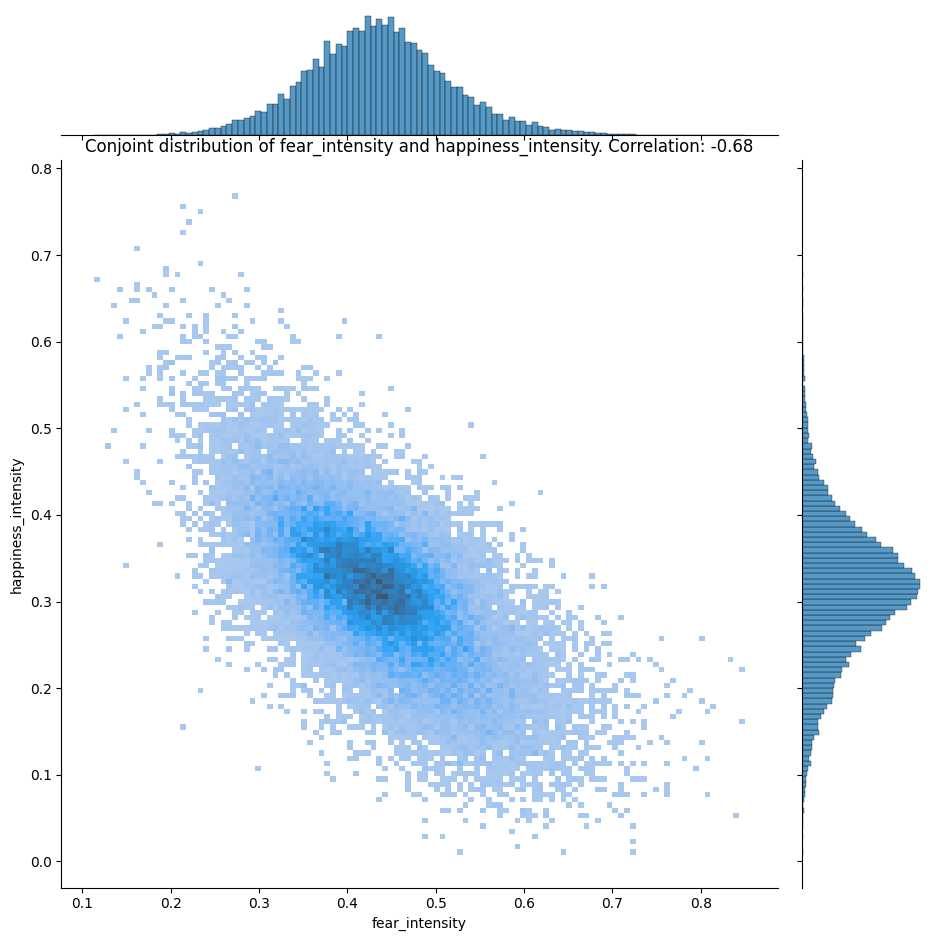
\includegraphics[scale=0.23]{./img/conjoint_distribution_fear_intensity_happiness_intensity.png}
\end{center}

Les distributions sont peu superposées, et la distribution conjointe présente une
anti-corrélation importante (-0.68). On peut donc en conclure que les deux variables jouent
un rôle oppposé dans la détermination du sentiment de l'internaute et que
généralement seule l'une d'entre elles aura une valeur élevée. Si les deux ont une
valeur similaire, l'internaute pourra être associé à un sentiment neutre.

\subsection*{fear vs sadness}

La représentation conjointe des distributions et la représentation de la
distribution conjointe des variables
\textit{fear\_intensity} et \textit{sadness\_intensity}
sont les suivantes :

\begin{center}
    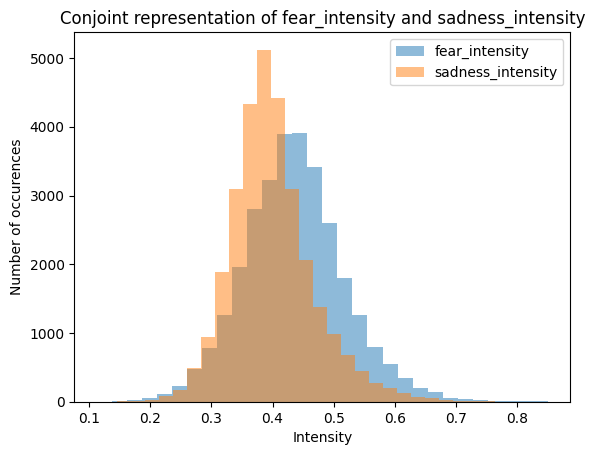
\includegraphics[scale=0.39]{./img/conjoint_representation_fear_intensity_sadness_intensity.png}
    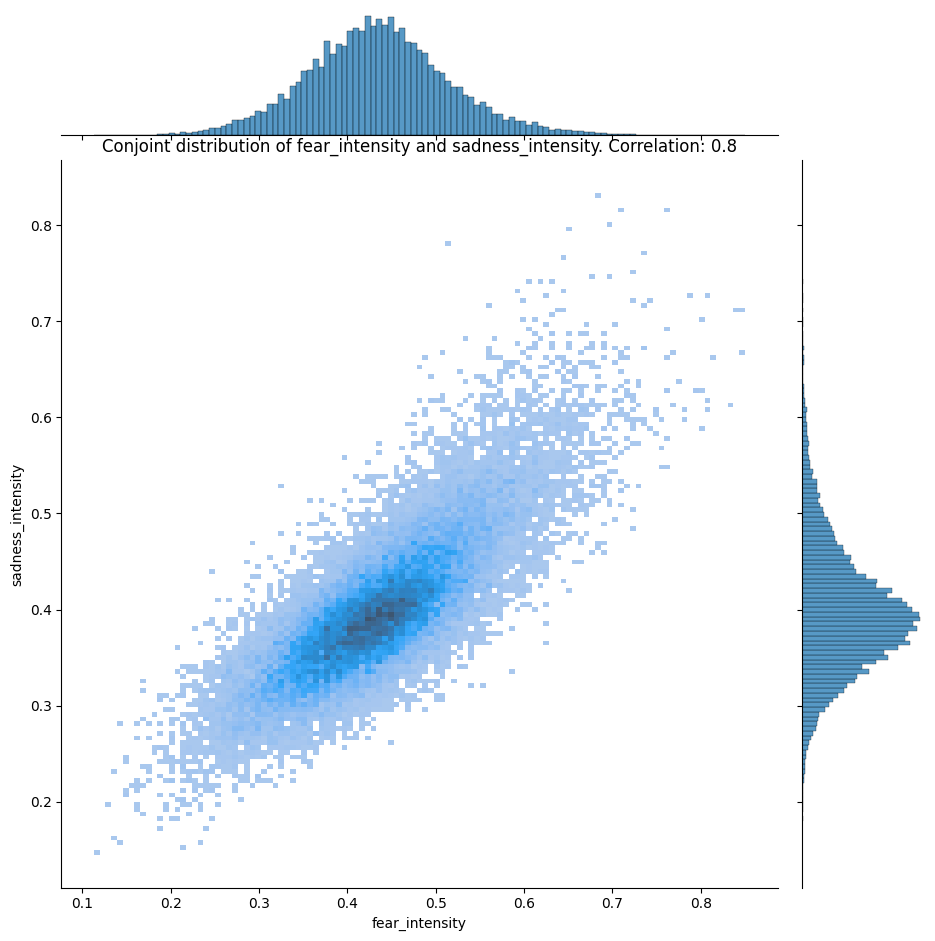
\includegraphics[scale=0.23]{./img/conjoint_distribution_fear_intensity_sadness_intensity.png}
\end{center}

Les distributions sont très superposées, et la distribution conjointe présente une
corrélation très importante (0.8). On peut donc en conclure que les deux variables jouent
un rôle équivalent dans la détermination du sentiment de l'internaute et que
généralement les deux auront une valeur élevée ou faible en même temps. Dans le cas de
la peur et de la tristesse, on imagine que l'internaute sera associé à un sentiment négatif
si les deux variables ont une valeur élevée et à un sentiment positif si les deux variables
ont une valeur faible.

\subsection*{happiness vs sadness}

La représentation conjointe des distributions et la représentation de la
distribution conjointe des variables
\textit{happiness\_intensity} et \textit{sadness\_intensity}
sont les suivantes :

\begin{center}
    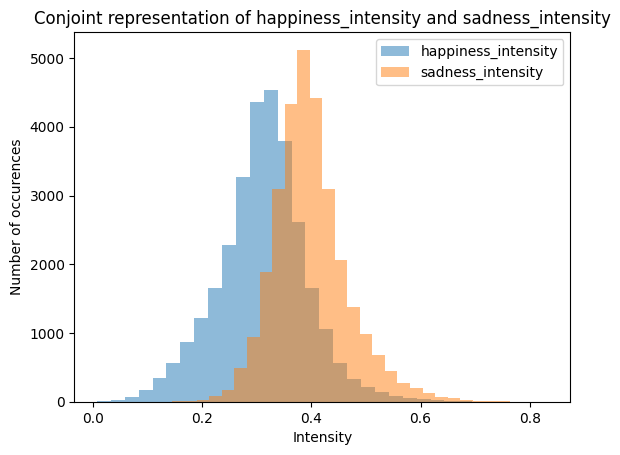
\includegraphics[scale=0.39]{./img/conjoint_representation_happiness_intensity_sadness_intensity.png}
    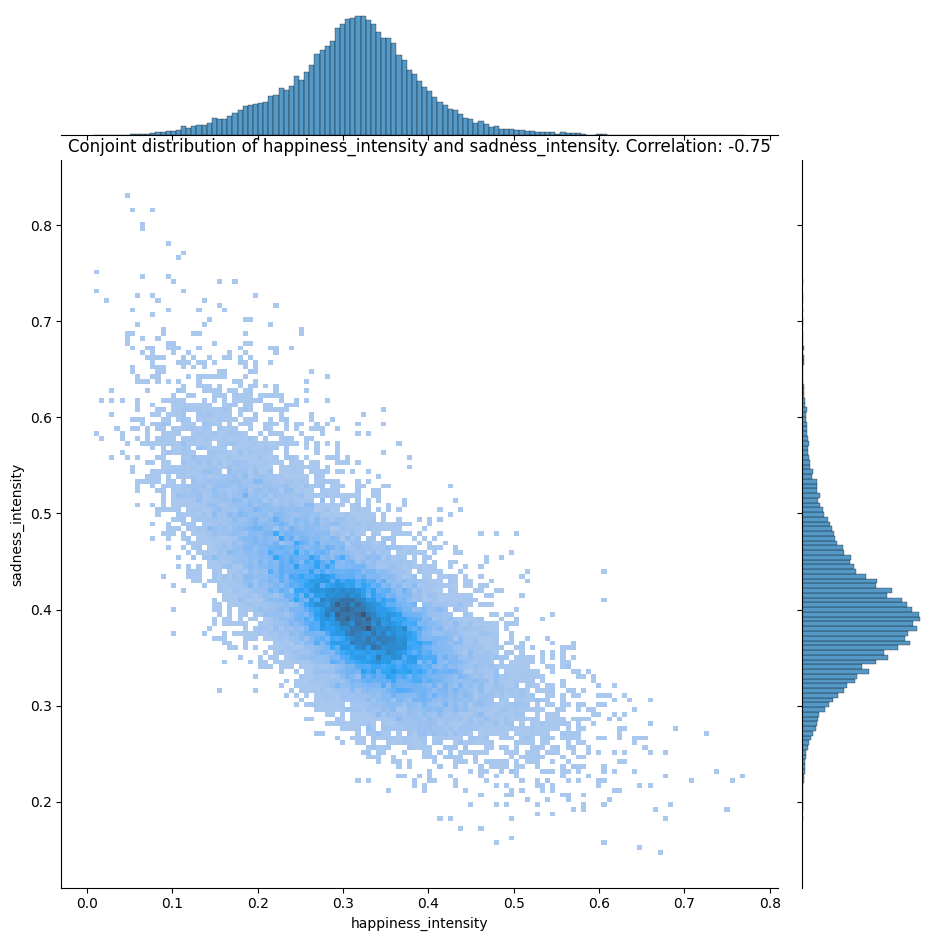
\includegraphics[scale=0.23]{./img/conjoint_distribution_happiness_intensity_sadness_intensity.png}
\end{center}

Les distributions sont moyennement superposées, et la distribution conjointe présente une
forte anti-corrélation (-0.75). On peut donc en conclure que les deux variables jouent
un rôle plutôt antagoniste dans la détermination du sentiment de l'internaute et que
la plupart du temps, seule l'une d'entre elles aura une valeur élevée. Si les deux ont une
valeur similaire, l'internaute pourra être associé à un sentiment neutre.

\subsection*{valence vs anger}

La représentation conjointe des distributions et la représentation de la
distribution conjointe des variables
\textit{valence\_intensity} et \textit{anger\_intensity}
sont les suivantes :

\begin{center}
    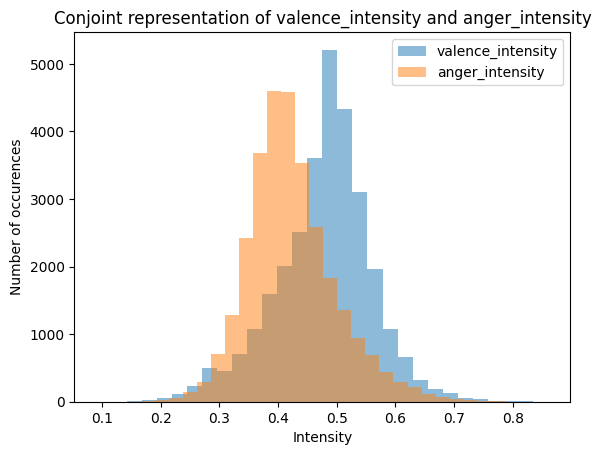
\includegraphics[scale=0.39]{./img/conjoint_representation_valence_intensity_anger_intensity.png}
    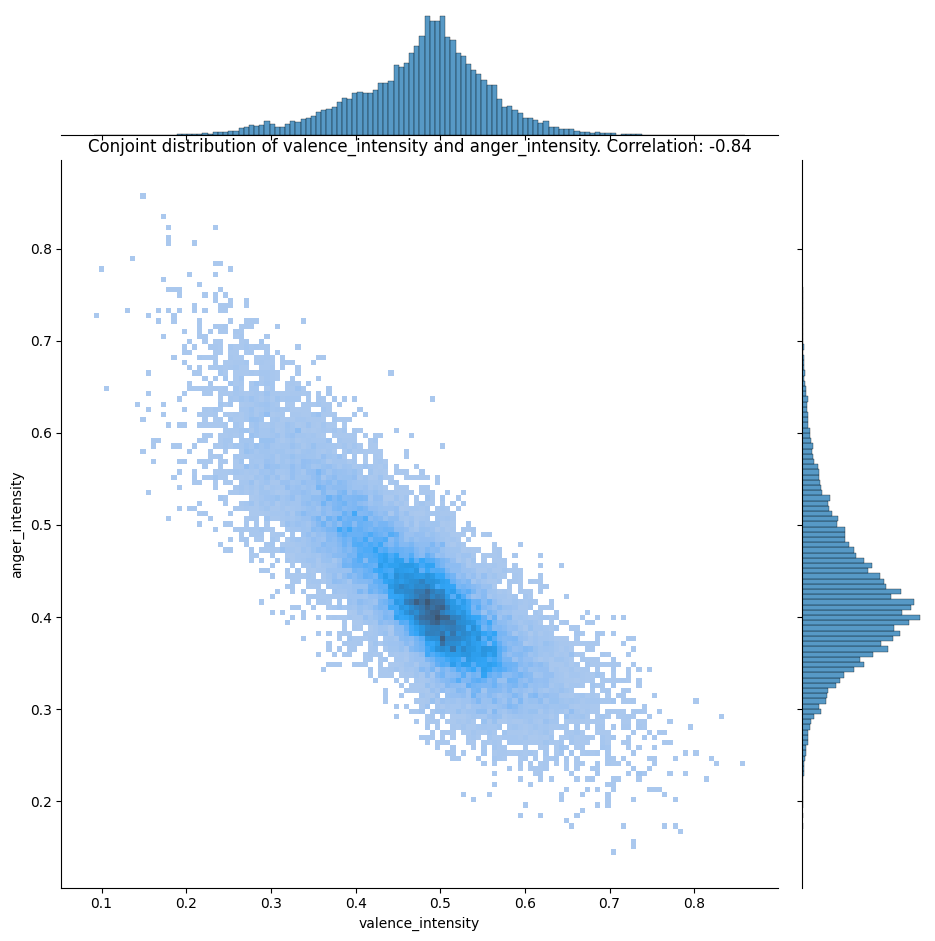
\includegraphics[scale=0.23]{./img/conjoint_distribution_valence_intensity_anger_intensity.png}
\end{center}

Les distributions sont assez peu superposées, et la distribution conjointe présente une
anti-corrélation extrêmement haute (-0.84). On peut donc en conclure que les deux variables jouent
un rôle complètement antagoniste dans la détermination du sentiment de l'internaute et que
la plupart du temps, seule l'une d'entre elles aura une valeur élevée. Si les deux ont une
valeur similaire, l'internaute pourra être associé à un sentiment neutre.
Il pourra être associé à un sentiment positif si la valence est élevée, et 
à un sentiment négatif si la colère est élevée.

\subsection*{valence vs fear}

La représentation conjointe des distributions et la représentation de la
distribution conjointe des variables
\textit{valence\_intensity} et \textit{fear\_intensity}
sont les suivantes :

\begin{center}
    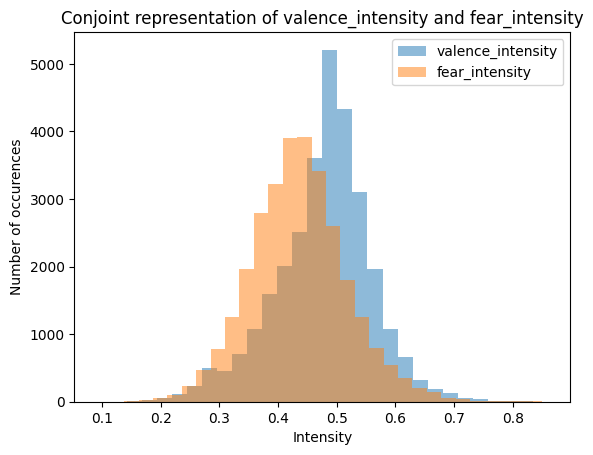
\includegraphics[scale=0.39]{./img/conjoint_representation_valence_intensity_fear_intensity.png}
    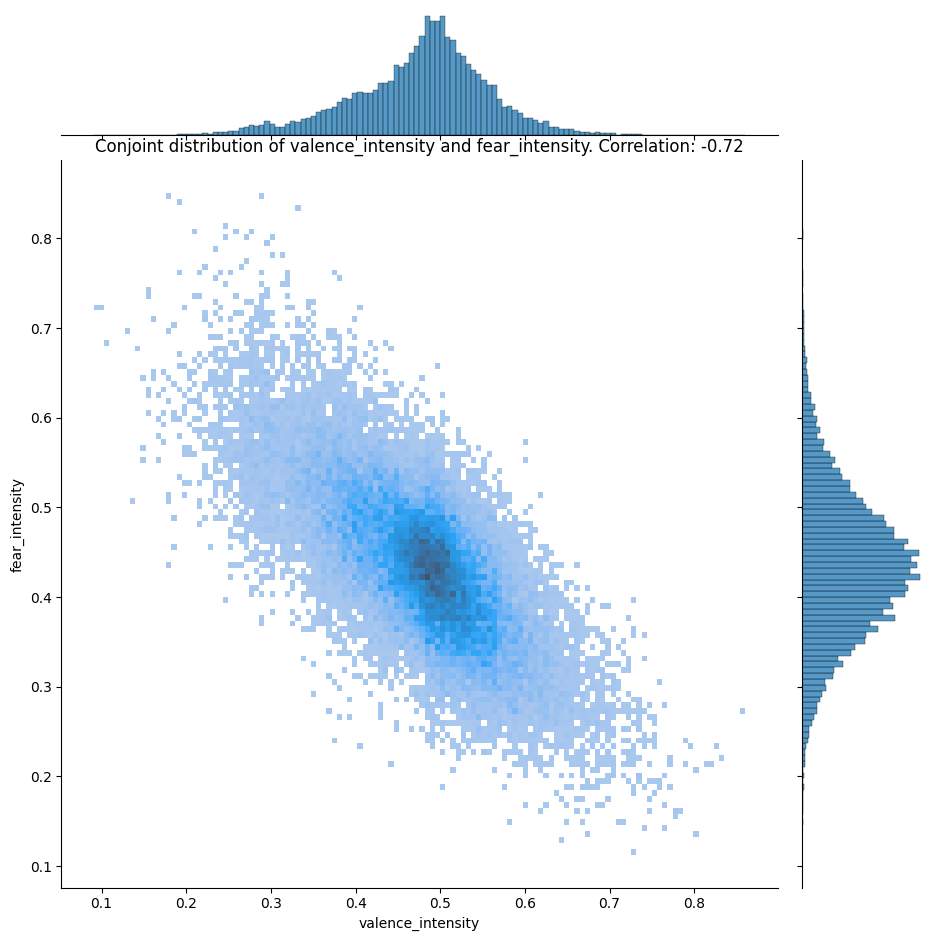
\includegraphics[scale=0.23]{./img/conjoint_distribution_valence_intensity_fear_intensity.png}
\end{center}

Les distributions sont plutôt superposées et la distribution conjointe présente une
anti-corrélation importante (-0.72). On peut donc en conclure que les deux variables jouent
un rôle plutôt antagoniste dans la détermination du sentiment de l'internaute et que
la plupart du temps, seule l'une d'entre elles aura une valeur élevée. Si les deux ont une
valeur similaire, l'internaute pourra être associé à un sentiment neutre.

\subsection*{valence vs happiness}

La représentation conjointe des distributions et la représentation de la
distribution conjointe des variables
\textit{valence\_intensity} et \textit{happiness\_intensity}
sont les suivantes :

\begin{center}
    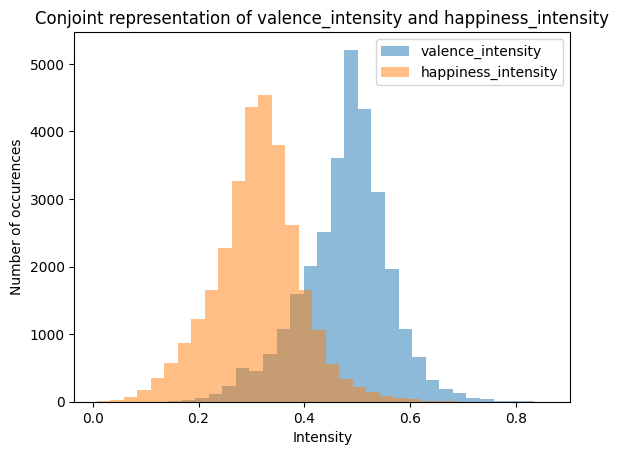
\includegraphics[scale=0.39]{./img/conjoint_representation_valence_intensity_happiness_intensity.png}
    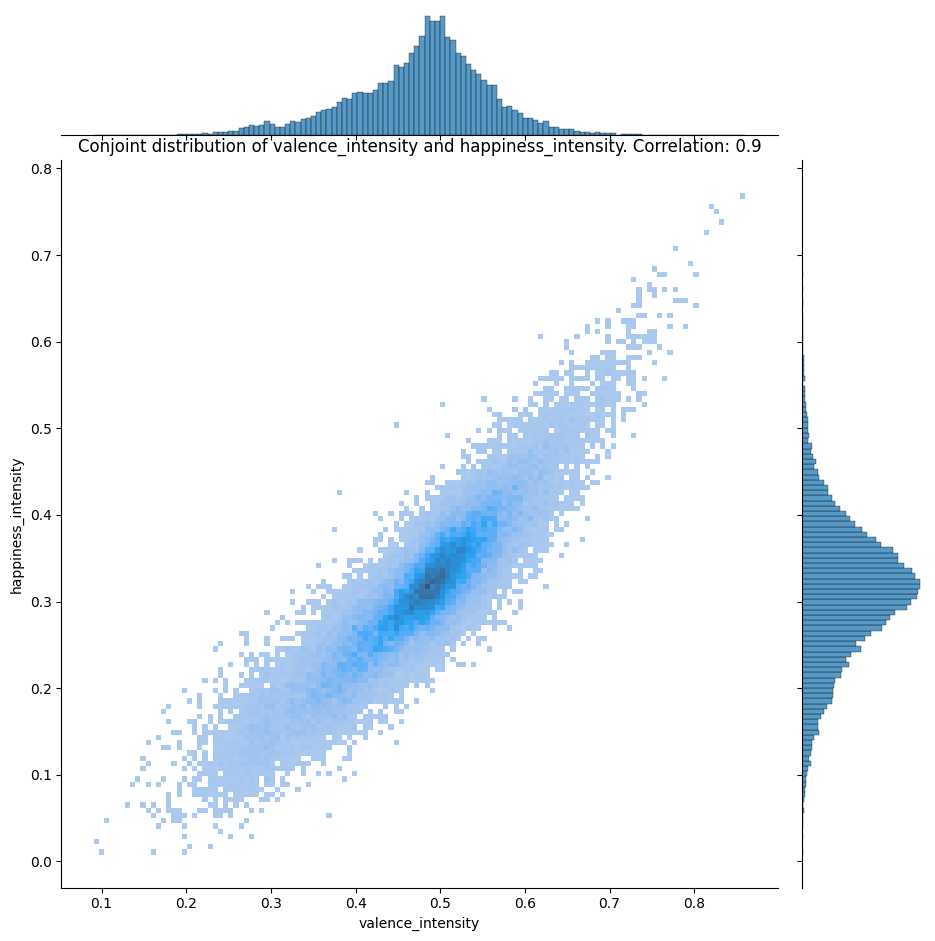
\includegraphics[scale=0.23]{./img/conjoint_distribution_valence_intensity_happiness_intensity.png}
\end{center}

Les distributions sont peu superposées, et la distribution conjointe présente une corrélation
extrêmement haute (0.9). On peut donc en conclure que les deux variables jouent
un rôle complètement similaire dans la détermination du sentiment de l'internaute et que
la plupart du temps, les deux auront une valeur élevée ou faible en même temps. Dans ce cas
précis, on imagine que l'internaute sera associé à un sentiment positif si les deux variables
ont une valeur élevée et à un sentiment négatif si les deux variables ont une valeur faible.

\subsection*{valence vs sadness}

La représentation conjointe des distributions et la représentation de la
distribution conjointe des variables
\textit{valence\_intensity} et \textit{sadness\_intensity}
sont les suivantes :

\begin{center}
    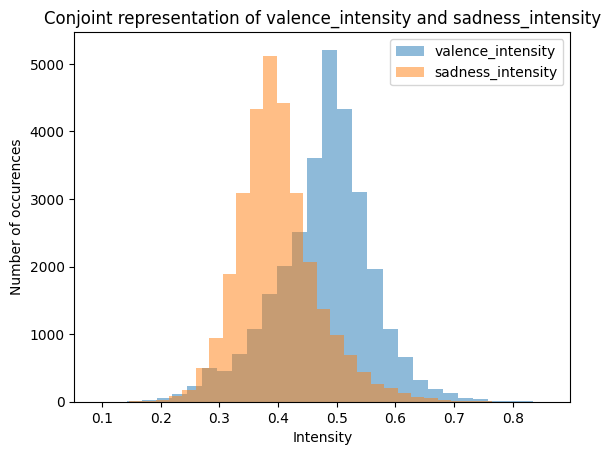
\includegraphics[scale=0.39]{./img/conjoint_representation_valence_intensity_sadness_intensity.png}
    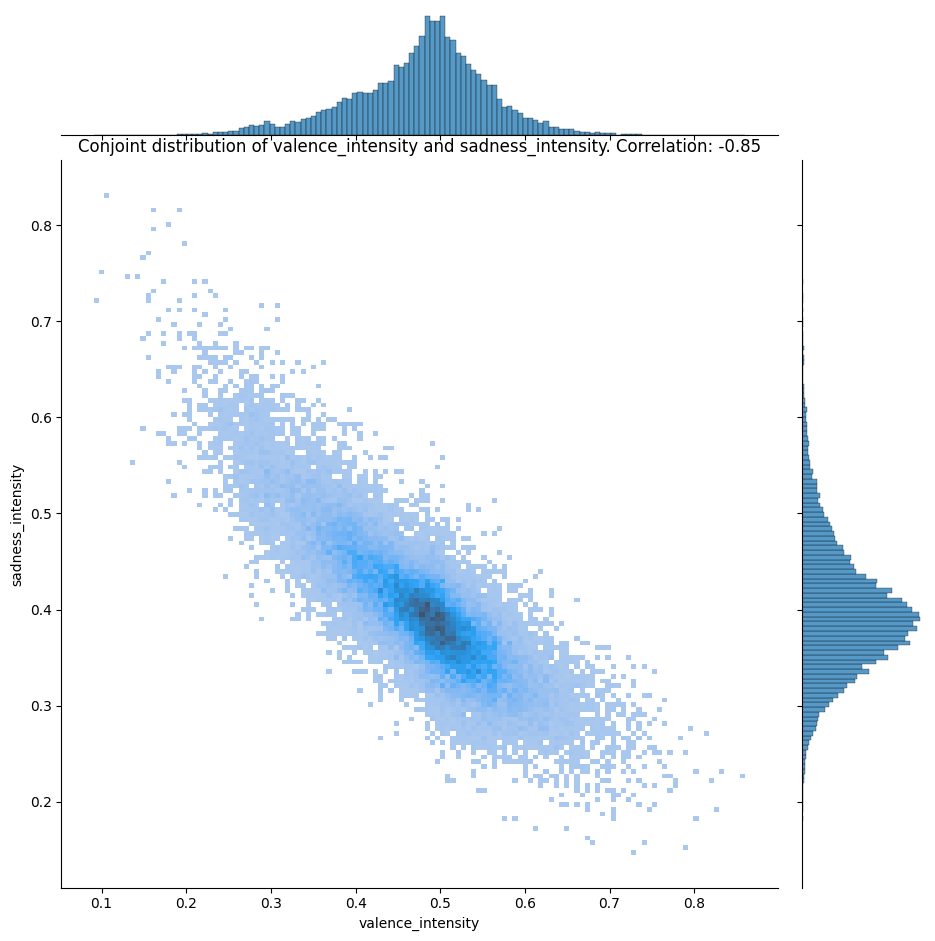
\includegraphics[scale=0.23]{./img/conjoint_distribution_valence_intensity_sadness_intensity.png}
\end{center}

Les distributions sont moyennement superposées, et la distribution conjointe présente une très
forte anti-corrélation (-0.85). On peut donc en conclure que les deux variables jouent
un rôle plutôt antagoniste dans la détermination du sentiment de l'internaute et que
la plupart du temps, seule l'une d'entre elles aura une valeur élevée 
(par rapport aux valeurs prises par cette variable en particulier). Si les deux ont une
valeur similaire, l'internaute pourra être associé à un sentiment neutre tandis que
si la valence est élevée (environ 0.6), l'internaute sera associé à un sentiment positif et
si la tristesse est élevée (environ 0.5), l'internaute sera associé à un sentiment négatif.


\newpage

\section*{Question 2}

\subsection*{Méthode}

Pour former les clusters, nous avons utilisé la fonction \textit{KMeans} de la librairie 
\textit{scikit-learn}. La projection des données dans un espace de dimension 2 a été réalisée
avec la fonction \textit{UMAP} de la librairie \textit{umap}. 

Nous avons donc roulé l'algorithme de clustering avec un nombre de clusters variant de 2 à 10.

\subsection*{Résultats}

Voici les graphiques obtenus pour les différents nombres de clusters.

\subsubsection*{2 clusters}

\begin{center}
    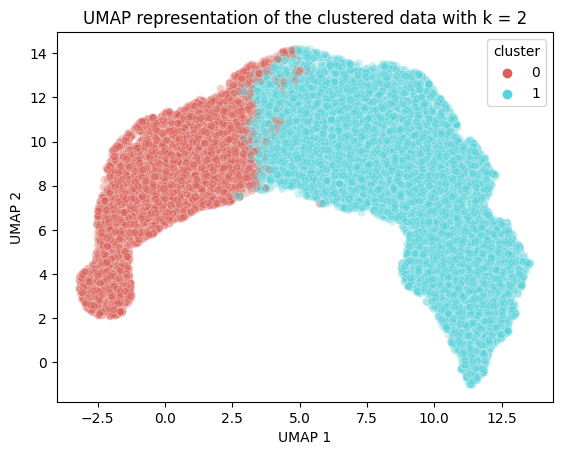
\includegraphics[scale=0.5]{./img/umap_2.png}
\end{center}

\subsubsection*{3 clusters}

\begin{center}
    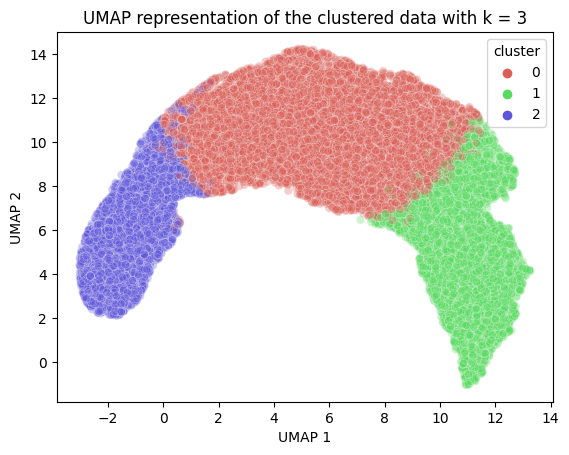
\includegraphics[scale=0.5]{./img/umap_3.png}
\end{center}

\subsubsection*{4 clusters}

\begin{center}
    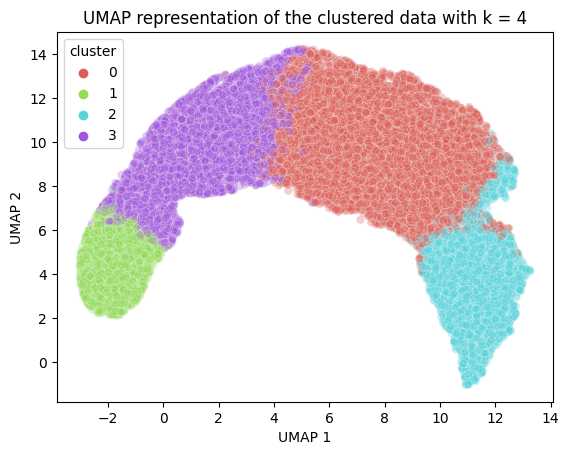
\includegraphics[scale=0.5]{./img/umap_4.png}
\end{center}

\subsubsection*{5 clusters}

\begin{center}
    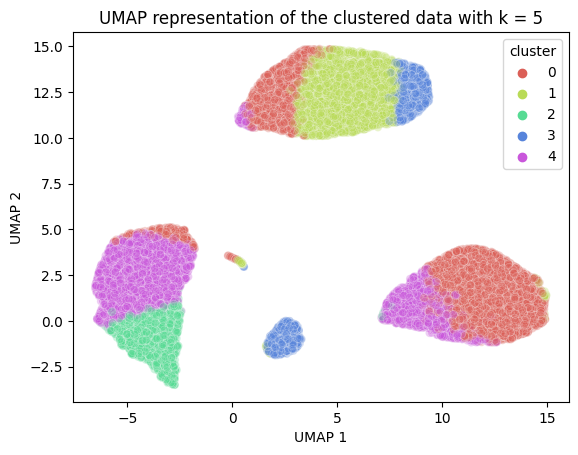
\includegraphics[scale=0.5]{./img/umap_5.png}
\end{center}

\subsubsection*{6 clusters}

\begin{center}
    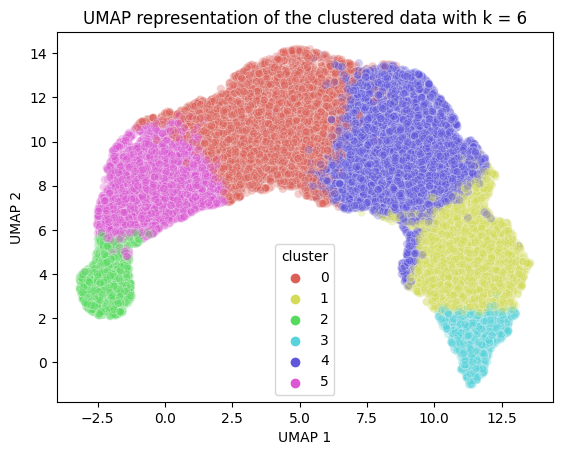
\includegraphics[scale=0.5]{./img/umap_6.png}
\end{center}

\subsubsection*{7 clusters}

\begin{center}
    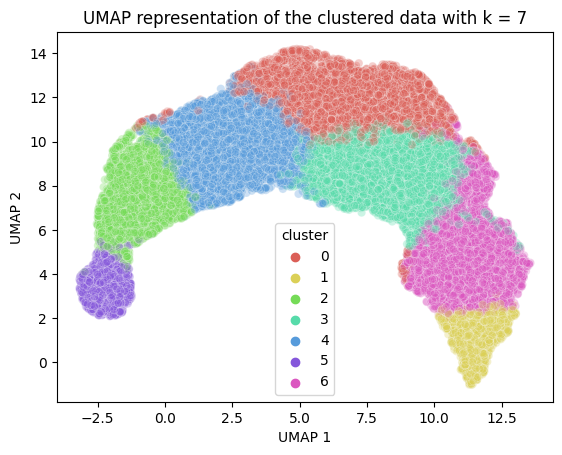
\includegraphics[scale=0.5]{./img/umap_7.png}
\end{center}

\subsubsection*{8 clusters}

\begin{center}
    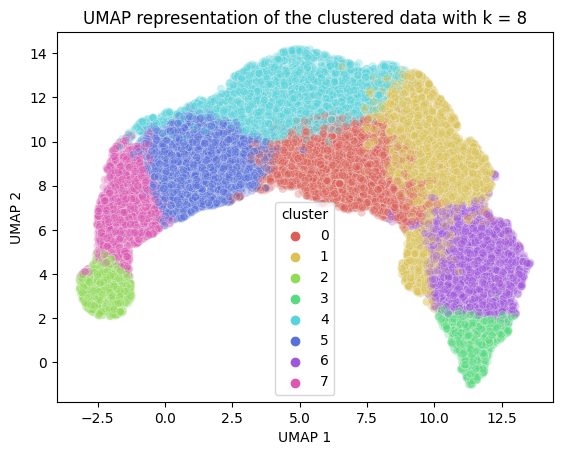
\includegraphics[scale=0.5]{./img/umap_8.png}
\end{center}

\subsubsection*{9 clusters}

\begin{center}
    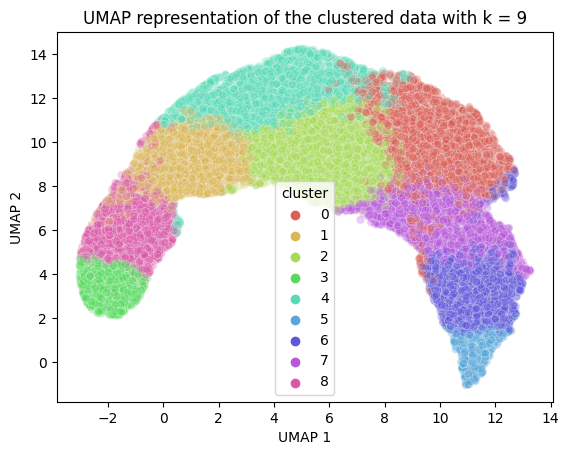
\includegraphics[scale=0.5]{./img/umap_9.png}
\end{center}

\subsubsection*{10 clusters}

\begin{center}
    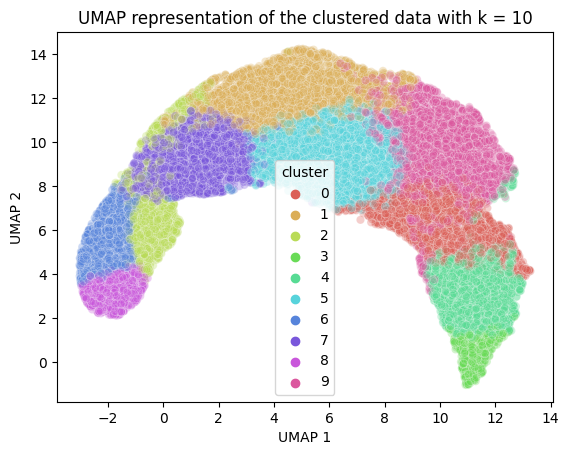
\includegraphics[scale=0.5]{./img/umap_10.png}
\end{center}

\subsection*{Interprétation}

On constate d'abord que les données elles-mêmes forment une structure assez agrégée.

On remarque que globalement, les clusters sont assez mal séparés et toujours en contact
les uns avec les autres. Mais ces résultats sont ceux attendus au vu de la structure des
données et forment quand même des ensembles de forme assez cohérente.

La taille des clusters diminue à mesure que le nombre de clusters augmente, ce qui est
logique car on divise les données en plus de clusters. Également, la taille des clusters
peut être inégale même au sein d'un même clustering. Par exemple, pour le cas avec 2 clusters,
le cluster de gauche contient plus de deux fois moins de données que le cluster de droite.
\newpage

\section*{Question 3 : métriques de séparation des clusters}

\subsection*{Méthode}

Pour calculer le score silhouette, nous avons utilisé la fonction 
\textit{silhouette\_score} de la librairie \textit{scikit-learn} et 
pour calculer les overlaps, nous avons implémenté des fonctions
\textit{distance\_intra\_classe} et \textit{distance\_inter\_classe}
ainsi qu'une fonction \textit{overlap} qui utilise les deux premières.

Nous avons fait attention a ne bien utiliser que les 5 features disponibles
dans les données et de mettre de côté le \textit{sentiment} et le \textit{cluster}
pour le calcul de ces métriques.

\subsection*{Résultats}

Voici les résultats obtenus pour les 2 mesures de séparation des clusters
pour les différents nombres de clusters.

\subsubsection*{2 clusters}

\noindent Score silhouette : 0.43 \\\\
Overlaps 2 à 2 :\\

\begin{center}
\begin{tabular}{|c|c|c|}
\hline
& C1 & C2 \\
\hline
C1 & - & 4.4 \\
\hline
C2 & - & - \\  
\hline
\end{tabular}
\end{center}

\subsubsection*{3 clusters}

\noindent Score silhouette : 0.34 \\\\
Overlaps 2 à 2 :\\

\begin{center}
\begin{tabular}{|c|c|c|c|}
\hline
& C1 & C2 & C3 \\
\hline
C1 & - & 4.49 & 3.38 \\
\hline
C2 & - & - & 1.74 \\
\hline
C3 & - & - & - \\   
\hline
\end{tabular} 
\end{center} 

\subsubsection*{4 clusters}

\noindent Score silhouette : 0.30 \\\\
Overlaps 2 à 2 :\\

\begin{center}
\begin{tabular}{|c|c|c|c|c|}
\hline
& C1 & C2 & C3 & C4 \\
\hline
C1 & - & 1.41 & 4.51 & 3.61 \\
\hline
C2 & - & - & 1.09 & 3.34 \\
\hline
C3 & - & - & - & 1.6 \\
\hline
C4 & - & - & - & - \\
\hline
\end{tabular} 
\end{center}

\subsubsection*{5 clusters}

\noindent Score silhouette : 0.26 \\\\
Overlaps 2 à 2 :\\

\begin{center}
\begin{tabular}{|c|c|c|c|c|c|}
\hline
& C1 & C2 & C3 & C4 & C5 \\
\hline
C1 & - & 3.45 & 1.7 & 1.36 & 4.5 \\
\hline
C2 & - & - & 1.02 & 3.36 & 1.47 \\
\hline
C3 & - & - & - & 0.82 & 4.21 \\
\hline
C4 & - & - & - & - & 0.98 \\
\hline
C5 & - & - & - & - & - \\
\hline
\end{tabular} 
\end{center}

\subsubsection*{6 clusters}

\noindent Score silhouette : 0.22

\subsubsection*{7 clusters}

\noindent Score silhouette : 0.20

\subsubsection*{8 clusters}

\noindent Score silhouette : 0.20

\subsubsection*{9 clusters}

\noindent Score silhouette : 0.19

\subsubsection*{10 clusters}

\noindent Score silhouette : 0.19

\subsection*{Interprétation}

On constate que le score silhouette est maximal pour 2 clusters et
diminue constamment par la suite. Même le score maximal (0.43) 
est plus proche de 0 que de 1, ce qui indique que les clusters son
assez mal séparés. Les scores correspondants aux grands nombres de clusters 
sont encore plus faibles (proches de 0.2), ce qui indique un fort 
chevauchement entre les clusters.

Concernant les overlaps, les valeurs sont généralement bien au dessus de 1,
(souvent aux alentours de 3) ce qui va également dans le sens d'un fort
chevauchement entre les clusters. 

On constate cela dit que les overlaps moyens
diminuent à mesure que le nombre de clusters augmente, ce qui est logique
car on divise les données en plus de clusters et donc que tous les clusters
ne se touchent plus, étant séparés par d'autres clusters. Cela ne 
constitue pas une amélioration de la qualité du clustering pour autant,
puisque les clusters qui présentent un overlap inférieur à 1 sont très 
chevauchants avec tous leurs voisins : aucun cluster n'est donc vraiment séparé
de tous les autres à la fois.

Pour tenter de justifier ces résultats, on peut remarquer que les
3 groupes formés par les internautes présentant les 3 sentiments sont
très proches les uns des autres. Voici les overlaps 2 à 2 entre ces
3 groupes :\\

\begin{center}
\begin{tabular}{|c|c|c|c|}
\hline
& -1 & 0 & 1 \\
\hline
-1 & - & 17.98 & 19.64 \\
\hline
0 & - & - & 32.09 \\
\hline
1 & - & - & - \\
\hline
\end{tabular}
\end{center}

Ces overlaps étant très élevés, on comprend que les groupes puissent être
difficiles à retrouver avec une méthode de clustering.

\newpage

\section*{Question 3 : cas particulier avec 3 clusters}

\subsection*{Méthode}

Pour mesurer si les clusters retrouvés correspondent effectivement,
aux internautes présentant les 3 sentiments, nous avons utilisé les critères
de précision, rappel et F1-score.

Pour calculer ces métriques efficacement, nous avons commencé par remplir
une table de contingence qui contient le nombre d'éléments de chaque classe
prédite pour chaque classe réelle comme suit :\\

\begin{center}
\begin{tabular}{|c|c|c|c|}
\hline
& -1 prédit & 0 prédit & 1 prédit \\
\hline
-1 réel & $N_{-1-1}$ & $N_{-10}$ & $N_{-11}$ \\
\hline
0 réel & $N_{0-1}$ & $N_{00}$ & $N_{01}$ \\
\hline
1 réel & $N_{1-1}$ & $N_{10}$ & $N_{11}$ \\
\hline
\end{tabular}
\end{center}

Nous avons ensuite utilisé la combinatoire pour en déduire la matrice de
confusion correspondant à ce clustering. Elle contient les nombres de vrais positifs,
faux positifs, vrais négatifs et faux négatifs associés. 

Les calculer explicitement nous a permis de gagner en efficacité par 
rapport à la méthode naïve qui consiste à itérer sur toutes les paires 
possibles d'éléments et à les classer comme vrais positifs s'ils ont la même 
classe réelle et la même classe prédite, etc.

Nous avons ensuite utilisé ces valeurs pour calculer les métriques de précision,
de rappel et de F1-score.

Ne sachant pas quel cluster formé correspond à quel sentiment, nous avons
testé toutes les associations possibles et gardé la meilleure.

\subsection*{Résultats}

Voici les résultats obtenus pour la meilleure association de clusters
avec les sentiments réels 
(qui est dans notre cas $(C1, C2, C3) \rightarrow (-1, 0, 1)$).

\begin{itemize}
    \item Précision : 0.64
    \item Rappel : 0.55
    \item F1-score : 0.59
\end{itemize}

\subsection*{Interprétation}

Les résultats sont moyens, mais lorsqu'on les affiche on constate que 
les clusters sont bien localisés proches des groupes d'internautes 
correspondant aux 3 sentiments.

Nous considérons donc que les résultats sont bons dans la mesure où la tâche
de clustering est difficile et que les résultats obtenus sont cohérents avec 
ce que nous attendions.

\section*{Question 4}

\subsection*{Méthode}

Pour cette question, nous avons utilisé la bibliothèque \textit{scipy.cluster.hierarchy}
pour réaliser un clustering hiérarchique. Nous avons utilisé la distance euclidienne
et le lien de Ward (nous avons aussi testé avec les liens simple et moyen qui donnent
des résultats similaires).

Pour chaque nombre de cluster, nous avons utilisé une recherche dichotomique 
pour trouver le seuil qui donne le nombre de clusters recherché.

Les fonctions de calcul de score silhouette et d'overlap sont les mêmes que pour
la question 3.

\subsection*{Résultats}

Voici les dendrogrammes obtenus pour les différentes valeurs de seuil trouvées ainsi
que les résultats des mesures de séparation des clusters.

\subsubsection*{\underline{Seuil = 18}}
Pour un seuil de 18, on obtient 2 clusters.\\
Dendrogramme correspondant :

\begin{center}
    \includegraphics[scale=0.19]{./img/dendrogram\_with\_threshold\_18\_2\_clusters.png}
\end{center}

\noindent Score silhouette : 0.45\\\\
Overlaps 2 à 2 :\\

\begin{center}
\begin{tabular}{|c|c|c|}
\hline
& C1 & C2 \\
\hline
C1 & - & 5.56 \\
\hline
C2 & - & - \\
\hline
\end{tabular}
\end{center}

\subsubsection*{\underline{Seuil = 12}}
Pour un seuil de 12, on obtient 3 clusters.\\
Dendrogramme correspondant :

\begin{center}
    \includegraphics[scale=0.19]{./img/dendrogram\_with\_threshold\_12\_3\_clusters.png}
\end{center}

\noindent Score silhouette : 0.28\\\\
Overlaps 2 à 2 :\\

\begin{center}
\begin{tabular}{|c|c|c|c|}
\hline
& C1 & C2 & C3 \\
\hline
C1 & - & 6.0 & 2.9 \\
\hline
C2 & - & - & 12.84 \\
\hline
C3 & - & - & - \\
\hline
\end{tabular}
\end{center}


\subsubsection*{\underline{Seuil = 9}}
Pour un seuil de 9, on obtient 4 clusters.\\
Dendrogramme correspondant :

\begin{center}
    \includegraphics[scale=0.19]{./img/dendrogram\_with\_threshold\_9\_4\_clusters.png}
\end{center}

\noindent Score silhouette : 0.25\\\\
Overlaps 2 à 2 :\\

\begin{center}
\begin{tabular}{|c|c|c|c|c|}
\hline
& C1 & C2 & C3 & C4 \\
\hline
C1 & - & 6.0 & 1.34 & 2.48 \\
\hline
C2 & - & - & 1.77 & 8.87 \\
\hline
C3 & - & - & - & 5.45 \\
\hline
C4 & - & - & - & - \\
\hline
\end{tabular}
\end{center}

\subsubsection*{\underline{Seuil = 8}}
Pour un seuil de 8, on obtient 5 clusters.\\
Dendrogramme correspondant :

\begin{center}
    \includegraphics[scale=0.19]{./img/dendrogram\_with\_threshold\_8\_5\_clusters.png}
\end{center}

\noindent Score silhouette : 0.22\\\\
Overlaps 2 à 2 :\\

\begin{center}
\begin{tabular}{|c|c|c|c|c|c|}
\hline
& C1 & C2 & C3 & C4 & C5 \\
\hline
C1 & - & 6.8 & 6.08 & 1.0 & 1.7 \\
\hline
C2 & - & - & 2.48 & 0.9 & 1.29 \\
\hline
C3 & - & - & - & 1.77 & 8.87 \\
\hline
C4 & - & - & - & - & 5.45 \\
\hline
C5 & - & - & - & - & - \\
\hline
\end{tabular}
\end{center}

\subsubsection*{\underline{Seuil = 6.2}}
Pour un seuil de 6.2, on obtient 6 clusters.\\
Dendrogramme correspondant :

\begin{center}
    \includegraphics[scale=0.19]{./img/dendrogram\_with\_threshold\_6.2\_6\_clusters.png}
\end{center}

\noindent Score silhouette : 0.18\\\\
Overlaps 2 à 2 :\\

\begin{center}
\begin{tabular}{|c|c|c|c|c|c|c|}
\hline
& C1 & C2 & C3 & C4 & C5 & C6 \\
\hline
C1 & - & 6.8 & 4.88 & 5.81 & 1.0 & 1.7 \\
\hline
C2 & - & - & 1.93 & 2.47 & 0.9 & 1.29 \\
\hline
C3 & - & - & - & 10.76 & 1.42 & 6.13 \\
\hline
C4 & - & - & - & - & 1.76 & 6.01 \\
\hline
C5 & - & - & - & - & - & 5.45 \\
\hline
C6 & - & - & - & - & - & - \\
\hline
\end{tabular}
\end{center}

\subsubsection*{\underline{Seuil = 6}}
Pour un seuil de 6, on obtient 7 clusters.\\
Dendrogramme correspondant :

\begin{center}
    \includegraphics[scale=0.19]{./img/dendrogram\_with\_threshold\_6\_7\_clusters.png}
\end{center}

\noindent Score silhouette : 0.15\\\\

\subsubsection*{\underline{Seuil = 5}}
Pour un seuil de 5, on obtient 8 clusters.\\
Dendrogramme correspondant :

\begin{center}
    \includegraphics[scale=0.19]{./img/dendrogram\_with\_threshold\_5\_8\_clusters.png}
\end{center}

\noindent Score silhouette : 0.14\\\\

\subsubsection*{\underline{Seuil = 4.5}}
Pour un seuil de 4.5, on obtient 9 clusters.\\
Dendrogramme correspondant :

\begin{center}
    \includegraphics[scale=0.19]{./img/dendrogram\_with\_threshold\_4.5\_9\_clusters.png}
\end{center}

\noindent Score silhouette : 0.13\\\\

\subsubsection*{\underline{Seuil = 3.63}}
Pour un seuil de 3.63, on obtient 10 clusters.\\
Dendrogramme correspondant :

\begin{center}
    \includegraphics[scale=0.19]{./img/dendrogram\_with\_threshold\_3.63\_10\_clusters.png}
\end{center}

\noindent Score silhouette : 0.13\\\\
\subsection*{Interprétation}

Les résultats sont assez similaires à ceux obtenus avec l'algorithme KMeans. En effet, les valeurs
de score silhouette sont comprises entre 0.13 et 0.45, ce qui est assez mauvais, et les overlaps
sont assez élevés, ce qui indique un fort chevauchement entre les clusters.

Ce n'est pas surprenant compte tenu du fait que la difficulté provient surtout de la structure
des données originelles et non de l'algorithme de clustering utilisé. N'importe quel algorithme
basé sur l'agglomération des internautes en fonction de leur distance euclidienne 
l'un par rapport à l'autre donnerait des résultats similaires.

\newpage

\section*{Question 5}

\subsection*{Méthode}

La méthode utilisée pour cette question est en tout point identique à celle utilisée pour la
deuxième partie de la question 3.

\subsection*{Résultats}

Voici les résultats obtenus pour la meilleure association de clusters
avec les sentiments réels 
(qui est dans notre cas $(C1, C2, C3) \rightarrow (1, 0, -1)$).

\begin{itemize}
    \item Précision : 0.75
    \item Rappel : 0.48
    \item F1-score : 0.59
\end{itemize}

\subsection*{Interprétation}

Les résultats sont similaires à ceux obtenus avec l'algorithme KMeans. Ils sont plutôt moyens bienque
correspondant à nos attentes, et confirment que, peu importe l'algorithme utilisé, 
la tâche de clustering est particulièrement difficile avec ces données. 

\end{document}
